\documentclass[tikz,border=6pt]{standalone}

\usepackage{amsmath}
\usepackage{array}
\usepackage{multirow}
\usepackage[table]{xcolor}
\usepackage[scaled=0.92]{helvet}
\renewcommand{\familydefault}{\sfdefault}
\usepackage{booktabs}

\usetikzlibrary{arrows.meta}

\definecolor{topblue}{RGB}{232,240,254}
\definecolor{helpergreen}{RGB}{230,244,234}
\definecolor{mainred}{RGB}{252,232,230}
\definecolor{headergray}{RGB}{248,248,248}
\definecolor{linegray}{RGB}{80,80,80}

\newcommand{\sfixed}[2]{signed fixed point $\langle #1.#2\rangle$}
\newcommand{\ufixed}[2]{unsigned fixed point $\langle #1.#2\rangle$}
\newcommand{\bitstring}[1]{bitstring $\langle #1\rangle$}

\tikzset{
  flow/.style={
    -{Latex[length=2.0mm]},
    draw=linegray,
    line width=0.45pt
  },
  box/.style={
    draw=linegray,
    rounded corners=1pt,
    inner sep=0pt,
    outer sep=0pt,
    align=center,
    font=\scriptsize
  }
}

\begin{document}
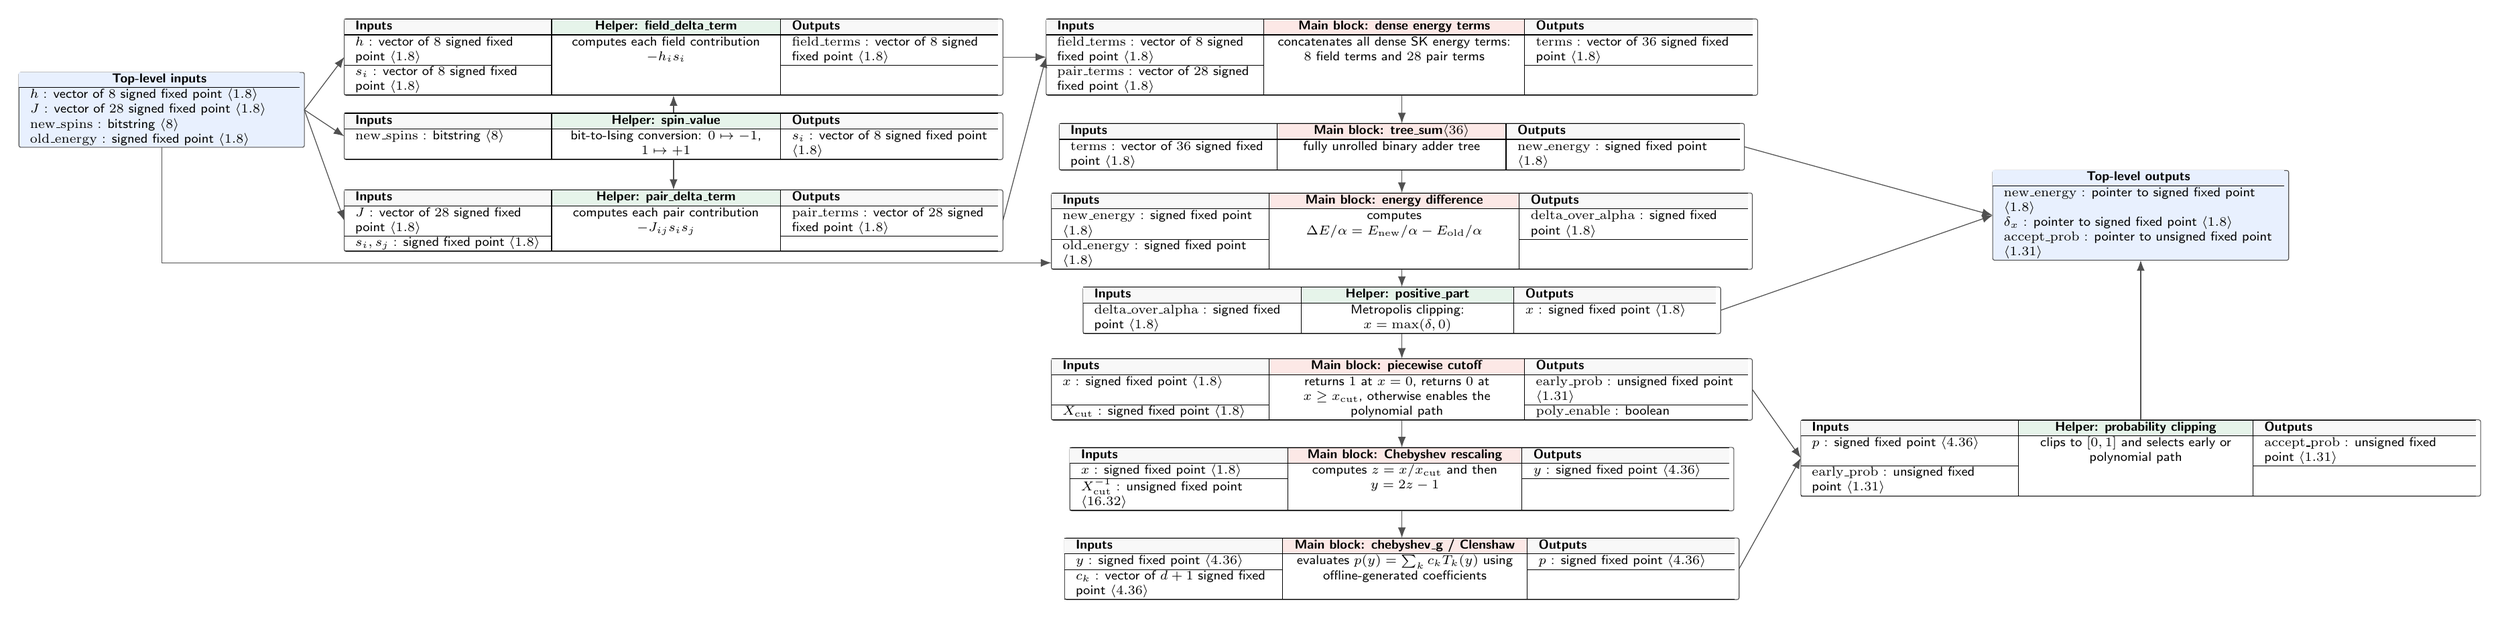
\begin{tikzpicture}[x=1cm,y=1cm]

% ---------------------------------------------------------------------------
% Top-level input and output boxes
% ---------------------------------------------------------------------------

\node[box, fill=topblue] (inputs) at (-3.5,0) {
\begin{tabular}{>{\raggedright\arraybackslash}p{4.9cm}}
\multicolumn{1}{c}{\cellcolor{topblue}\textbf{Top-level inputs}}\\
\hline
$h$ : vector of $8$ \sfixed{1}{8}\\
$J$ : vector of $28$ \sfixed{1}{8}\\
$\mathrm{new\_spins}$ : \bitstring{8}\\
$\mathrm{old\_energy}$ : \sfixed{1}{8}\\
\end{tabular}
};

\node[box, fill=topblue] (outputs) at (34,-2) {
\begin{tabular}{>{\raggedright\arraybackslash}p{5.1cm}}
\multicolumn{1}{c}{\cellcolor{topblue}\textbf{Top-level outputs}}\\
\hline
$\mathrm{new\_energy}$ : pointer to \sfixed{1}{8}\\
$\delta_x$ : pointer to \sfixed{1}{8}\\
$\mathrm{accept\_prob}$ : pointer to \ufixed{1}{31}\\
\end{tabular}
};

% ---------------------------------------------------------------------------
% Helper blocks
% ---------------------------------------------------------------------------

\node[box] (spin_values) at (6.2,-0.5) {
\begin{tabular}{>{\raggedright\arraybackslash}p{3.5cm}|>{\centering\arraybackslash}p{3.9cm}|>{\raggedright\arraybackslash}p{3.7cm}}
\hline
\cellcolor{headergray}\textbf{Inputs} &
\cellcolor{helpergreen}\textbf{Helper: spin\_value} &
\cellcolor{headergray}\textbf{Outputs}\\
\hline
$\mathrm{new\_spins}$ : \bitstring{8} &
bit-to-Ising conversion: $0\mapsto -1$, $1\mapsto +1$ &
$s_i$ : vector of $8$ \sfixed{1}{8}\\
\hline
\end{tabular}
};

\node[box] (field_terms) at (6.2,1.0) {
\begin{tabular}{>{\raggedright\arraybackslash}p{3.5cm}|>{\centering\arraybackslash}p{3.9cm}|>{\raggedright\arraybackslash}p{3.7cm}}
\hline
\cellcolor{headergray}\textbf{Inputs} &
\cellcolor{helpergreen}\textbf{Helper: field\_delta\_term} &
\cellcolor{headergray}\textbf{Outputs}\\
\hline
$h$ : vector of $8$ \sfixed{1}{8} &
\multirow{2}{=}{\centering computes each field contribution $-h_i s_i$} &
$\mathrm{field\_terms}$ : vector of $8$ \sfixed{1}{8}\\
\cline{1-1}\cline{3-3}
$s_i$ : vector of $8$ \sfixed{1}{8} & & \\
\hline
\end{tabular}
};

\node[box] (pair_terms_helper) at (6.2,-2.1) {
\begin{tabular}{>{\raggedright\arraybackslash}p{3.5cm}|>{\centering\arraybackslash}p{3.9cm}|>{\raggedright\arraybackslash}p{3.7cm}}
\hline
\cellcolor{headergray}\textbf{Inputs} &
\cellcolor{helpergreen}\textbf{Helper: pair\_delta\_term} &
\cellcolor{headergray}\textbf{Outputs}\\
\hline
$J$ : vector of $28$ \sfixed{1}{8} &
\multirow{2}{=}{\centering computes each pair contribution $-J_{ij}s_i s_j$} &
$\mathrm{pair\_terms}$ : vector of $28$ \sfixed{1}{8}\\
\cline{1-1}\cline{3-3}
$s_i,s_j$ : \sfixed{1}{8} & & \\
\hline
\end{tabular}
};

% ---------------------------------------------------------------------------
% Main dense-energy path
% ---------------------------------------------------------------------------

\node[box] (energy_terms) at (20.0,1.0) {
\begin{tabular}{>{\raggedright\arraybackslash}p{3.7cm}|>{\centering\arraybackslash}p{4.5cm}|>{\raggedright\arraybackslash}p{3.9cm}}
\hline
\cellcolor{headergray}\textbf{Inputs} &
\cellcolor{mainred}\textbf{Main block: dense energy terms} &
\cellcolor{headergray}\textbf{Outputs}\\
\hline
$\mathrm{field\_terms}$ : vector of $8$ \sfixed{1}{8} &
\multirow{2}{=}{\centering concatenates all dense SK energy terms: $8$ field terms and $28$ pair terms} &
$\mathrm{terms}$ : vector of $36$ \sfixed{1}{8}\\
\cline{1-1}\cline{3-3}
$\mathrm{pair\_terms}$ : vector of $28$ \sfixed{1}{8} & & \\
\hline
\end{tabular}
};

\node[box] (tree) at (20,-0.7) {
\begin{tabular}{>{\raggedright\arraybackslash}p{3.7cm}|>{\centering\arraybackslash}p{3.9cm}|>{\raggedright\arraybackslash}p{4.0cm}}
\hline
\cellcolor{headergray}\textbf{Inputs} &
\cellcolor{mainred}\textbf{Main block: tree\_sum$\langle 36\rangle$} &
\cellcolor{headergray}\textbf{Outputs}\\
\hline
$\mathrm{terms}$ : vector of $36$ \sfixed{1}{8} &
fully unrolled binary adder tree &
$\mathrm{new\_energy}$ : \sfixed{1}{8}\\
\hline
\end{tabular}
};

\node[box] (delta) at (20,-2.3) {
\begin{tabular}{>{\raggedright\arraybackslash}p{3.7cm}|>{\centering\arraybackslash}p{4.3cm}|>{\raggedright\arraybackslash}p{3.9cm}}
\hline
\cellcolor{headergray}\textbf{Inputs} &
\cellcolor{mainred}\textbf{Main block: energy difference} &
\cellcolor{headergray}\textbf{Outputs}\\
\hline
$\mathrm{new\_energy}$ : \sfixed{1}{8} &
\multirow{2}{=}{\centering computes $\Delta E/\alpha=E_{\rm new}/\alpha-E_{\rm old}/\alpha$} &
$\mathrm{delta\_over\_alpha}$ : \sfixed{1}{8}\\
\cline{1-1}\cline{3-3}
$\mathrm{old\_energy}$ : \sfixed{1}{8} & & \\
\hline
\end{tabular}
};

\node[box] (positive) at (20,-3.8) {
\begin{tabular}{>{\raggedright\arraybackslash}p{3.7cm}|>{\centering\arraybackslash}p{3.6cm}|>{\raggedright\arraybackslash}p{3.4cm}}
\hline
\cellcolor{headergray}\textbf{Inputs} &
\cellcolor{helpergreen}\textbf{Helper: positive\_part} &
\cellcolor{headergray}\textbf{Outputs}\\
\hline
$\mathrm{delta\_over\_alpha}$ : \sfixed{1}{8} &
Metropolis clipping: $x=\max(\delta,0)$ &
$x$ : \sfixed{1}{8}\\
\hline
\end{tabular}
};

% ---------------------------------------------------------------------------
% Probability path
% ---------------------------------------------------------------------------

\node[box] (cutoff) at (20.0,-5.3) {
\begin{tabular}{>{\raggedright\arraybackslash}p{3.7cm}|>{\centering\arraybackslash}p{4.4cm}|>{\raggedright\arraybackslash}p{3.8cm}}
\hline
\cellcolor{headergray}\textbf{Inputs} &
\cellcolor{mainred}\textbf{Main block: piecewise cutoff} &
\cellcolor{headergray}\textbf{Outputs}\\
\hline
$x$ : \sfixed{1}{8} &
\multirow{2}{=}{\centering returns $1$ at $x=0$, returns $0$ at $x\ge x_{\rm cut}$, otherwise enables the polynomial path} &
$\mathrm{early\_prob}$ : \ufixed{1}{31}\\
\cline{1-1}\cline{3-3}
$X_{\rm cut}$ : \sfixed{1}{8} & & $\mathrm{poly\_enable}$ : boolean\\
\hline
\end{tabular}
};

\node[box] (rescale) at (20,-7.0) {
\begin{tabular}{>{\raggedright\arraybackslash}p{3.7cm}|>{\centering\arraybackslash}p{4.0cm}|>{\raggedright\arraybackslash}p{3.5cm}}
\hline
\cellcolor{headergray}\textbf{Inputs} &
\cellcolor{mainred}\textbf{Main block: Chebyshev rescaling} &
\cellcolor{headergray}\textbf{Outputs}\\
\hline
$x$ : \sfixed{1}{8} &
\multirow{2}{=}{\centering computes $z=x/x_{\rm cut}$ and then $y=2z-1$} &
$y$ : \sfixed{4}{36}\\
\cline{1-1}\cline{3-3}
$X_{\rm cut}^{-1}$ : \ufixed{16}{32} & & \\
\hline
\end{tabular}
};

\node[box] (clenshaw) at (20,-8.7) {
\begin{tabular}{>{\raggedright\arraybackslash}p{3.7cm}|>{\centering\arraybackslash}p{4.2cm}|>{\raggedright\arraybackslash}p{3.5cm}}
\hline
\cellcolor{headergray}\textbf{Inputs} &
\cellcolor{mainred}\textbf{Main block: chebyshev\_g / Clenshaw} &
\cellcolor{headergray}\textbf{Outputs}\\
\hline
$y$ : \sfixed{4}{36} &
\multirow{2}{=}{\centering evaluates $p(y)=\sum_k c_k T_k(y)$ using offline-generated coefficients} &
$p$ : \sfixed{4}{36}\\
\cline{1-1}\cline{3-3}
$c_k$ : vector of $d+1$ \sfixed{4}{36} & & \\
\hline
\end{tabular}
};

\node[box] (probclip) at (34,-6.6) {
\begin{tabular}{>{\raggedright\arraybackslash}p{3.7cm}|>{\centering\arraybackslash}p{4.0cm}|>{\raggedright\arraybackslash}p{3.8cm}}
\hline
\cellcolor{headergray}\textbf{Inputs} &
\cellcolor{helpergreen}\textbf{Helper: probability clipping} &
\cellcolor{headergray}\textbf{Outputs}\\
\hline
$p$ : \sfixed{4}{36} &
\multirow{2}{=}{\centering clips to $[0,1]$ and selects early or polynomial path} &
$\mathrm{accept\_prob}$ : \ufixed{1}{31}\\
\cline{1-1}\cline{3-3}
$\mathrm{early\_prob}$ : \ufixed{1}{31} & & \\
\hline
\end{tabular}
};

% ---------------------------------------------------------------------------
% Straight arrows only
% ---------------------------------------------------------------------------

\draw[flow] (inputs.east) -- (spin_values.west);
\draw[flow] (inputs.east) -- (field_terms.west);
\draw[flow] (inputs.east) -- (pair_terms_helper.west);

\draw[flow] (spin_values.north) -- (field_terms.south);
\draw[flow] (spin_values.south) -- (pair_terms_helper.north);

\draw[flow] (field_terms.east) -- (energy_terms.west);
\draw[flow] (pair_terms_helper.east) -- (energy_terms.west);

\draw[flow] (energy_terms.south) -- (tree.north);
\draw[flow] (tree.south) -- (delta.north);
\draw[flow] (inputs.south) |- ([yshift=-0.6cm]delta.west);

\draw[flow] (tree.east) -- (outputs.west);
\draw[flow] (delta.south) -- (positive.north);
\draw[flow] (positive.east) -- (outputs.west);
\draw[flow] (positive.south) -- (cutoff.north);

\draw[flow] (cutoff.south) -- (rescale.north);
\draw[flow] (rescale.south) -- (clenshaw.north);
\draw[flow] (clenshaw.east) -- (probclip.west);
\draw[flow] (cutoff.east) -- (probclip.west);
\draw[flow] (probclip.north) -- (outputs.south);

\end{tikzpicture}
\end{document}
